\documentclass[a4paper]{article}
\usepackage{blindtext}
\usepackage{csvsimple}
\usepackage{graphicx}
\usepackage{placeins}
\usepackage{hyperref}


\title{Assignment 5}
\author{Baktash Ansari}
\date{\today}

\begin{document}  

\maketitle

\section{Attention exploration}

\subsection*{a.i.}
The attention weights \(\alpha\) can be interpreted as a categorical probability distribution because :

1. Each attention weight $\alpha_i$ is computed as the exponential of a key-query similarity score $(k_i^\top q)$, followed by a normalization factor. Since both the exponential function and the normalization factor (denominator) are non-negative, it ensures that each attention weight $\alpha_i$ is also non-negative. This property is essential for interpreting the attention weights as probabilities.

2. The attention weights are computed by dividing the exponential of each key-query similarity score by the sum of exponentials over all key-query similarity scores. This division by the sum ensures that the attention weights add up to 1, which is a fundamental property of probability distributions. Consequently, the attention weights represent the probabilities of selecting the corresponding value vectors based on the similarity between the query and the keys.

By satisfying both properties, the attention weights $\alpha$ can be interpreted as probabilities. They indicate the relative importance or relevance of each value vector in the context of the given query vector. The higher the attention weight, the more attention is assigned to the corresponding value vector during the computation of the output $c$, resembling a probabilistic selection process.

\subsection*{a.ii.}

As we see in above equations, for calculating $\alpha_i$ we have a probability that calculate over $(k_i^\top q)$ so when the value of $(k_j^\top q)$ for specific j becomes significantly high comparing other values, the probability becomes higher than others too.
Resulting in  a high value of $\alpha_j$ compared to the other $\alpha_i$ values which leads to categorical distribution $\alpha$ puts almost all of its weight on some $\alpha_j$

\subsection*{a.iii.}

Under the conditions where the categorical distribution $\alpha$ puts almost all of its weight on some $\alpha_j$, the output c will be predominantly influenced by the value vector \(V_j\). Since $\alpha_j$ carries a significantly larger weight compared to other $\alpha_i$ values, the value vector vj will contribute significantly more to the computation of the output c than the other value vectors. In other words, the output c will be heavily influenced by the value vector vj, reflecting the high importance placed on it by the attention mechanism.

\subsection*{a.iv.}
When the categorical distribution $\alpha$ puts almost all of its weight on a specific $\alpha_j$, it means that the attention mechanism is focusing heavily on a particular key-value pair. The output c will be predominantly influenced by the value vector associated with that key, indicating that the attention mechanism has identified a highly relevant and informative relationship between the query and that specific key-value pair.

\subsection*{b.i.}
To construct the matrix $M$ that can extract $v_a$ from the sum vector $s = v_a + v_b$, we can use the basis vectors $\{a_1, a_2, ..., a_m\}$. We create a matrix $M$ with the basis vectors as its columns, i.e., $M = [a_1, a_2, ..., a_m]$.


\( v_a = c_1a_1 + c_2a_2 + ... + c_ma_m \)

Now, let's denote the vector of weights $c$ as $c = [c_1, c_2, ..., c_m]$.

We can then show that $M$ multiplied by the sum vector $s$ will result in $v_a$:

$Ms = M(v_a + v_b) = M(c_1a_1 + c_2a_2 + ... + c_ma_m + v_b) = c_1Ma_1 + c_2Ma_2 + ... + c_mMa_m + Mv_b$

Since the matrix $M$ consists of the basis vectors $\{a_1, a_2, ..., a_m\}$, the term $Mv_b$ will be zero since the basis vectors for subspace $A$ and $B$ are orthogonal. Therefore, the equation simplifies to:

$Ms = c_1Ma_1 + c_2Ma_2 + ... + c_mMa_m = c_1a_1 + c_2a_2 + ... + c_ma_m = v_a$

Hence, we have shown that $M$ multiplied by the sum vector $s$ ($v_a + v_b$) equals $v_a$, which means $M$ can be used to extract $v_a$ from the sum vector.


\subsection*{b.ii.}

To find an expression for a query vector $q$ such that $c \approx \frac{1}{2} \cdot (v_a + v_b)$, we can take advantage of the given conditions: (1) all key vectors are orthogonal, and (2) all key vectors have a norm of 1.

First, let's consider the attention weights $\alpha_i$ for the two value vectors $v_a$ and $v_b$. Using Equation (2) from the initial question, we have:

\[
\alpha_i = \frac{{\exp(k_i^\top q)}}{{\exp(k_a^\top q) + \exp(k_b^\top q)}}
\]

Given that all key vectors are orthogonal, we have $k_a^\top k_b = 0$. Since the norm of each key vector is 1, we have $k_a^\top k_a = k_b^\top k_b = 1$.

Now, let's consider the numerator of the attention weight $\alpha_i$:

\[
\exp(k_i^\top q) = \exp\left((k_i^\top v_a + k_i^\top v_b)^\top q\right)
\]

Using the property of exponentiation, we can rewrite this as:

\[
\exp(k_i^\top q) = \exp((k_i^\top v_a)^\top q) \cdot \exp((k_i^\top v_b)^\top q) = \exp(v_a^\top k_i q) \cdot \exp(v_b^\top k_i q)
\]

Since the key vectors $k_a$ and $k_b$ are orthogonal, $v_a^\top k_b = 0$. Thus, the term $\exp(v_b^\top k_i q)$ does not depend on $v_a$, and vice versa for the term $\exp(v_a^\top k_i q)$.

Now, let's consider the denominator of the attention weight $\alpha_i$:

\[
\exp(k_a^\top q) + \exp(k_b^\top q) = \exp((k_a^\top v_a + k_a^\top v_b)^\top q) + \exp((k_b^\top v_a + k_b^\top v_b)^\top q)
\]

Using the same logic as before, we can separate the terms that depend on $v_a$ and $v_b$:

\[
\exp((k_a^\top v_a)^\top q) \cdot \exp((k_a^\top v_b)^\top q) + \exp((k_b^\top v_a)^\top q) \cdot \exp((k_b^\top v_b)^\top q)
\]

Since we want $c$ to be approximately equal to $\frac{1}{2} \cdot (v_a + v_b)$, we can assume that $v_a$ and $v_b$ have similar magnitudes. In this case, $\exp(v_a^\top k_i q)$ and $\exp(v_b^\top k_i q)$ will also have similar magnitudes. Similarly, the terms $\exp((k_a^\top v_a)^\top q) \cdot \exp((k_a^\top v_b)^\top q)$ and $\exp((k_b^\top v_a)^\top q) \cdot \exp((k_b^\top v_b)^\top q)$ will have similar magnitudes.

Now, let's consider the ratio of the attention weights:

\[
\alpha_i \approx \frac{{\exp(v_a^\top k_i q) \cdot \exp(v_b^\top k_i q)}}{{\exp((k_a^\top v_a)^\top q) \cdot \exp((k_b^\top v_b)^\top q) + \exp((k_a^\top v_b)^\top q) \cdot \exp((k_b^\top v_a)^\top q)}}
\]

As mentioned earlier, if $v_a$ and $v_b$ have similar magnitudes, the terms $\exp(v_a^\top k_i q)$ and $\exp(v_b^\top k_i q)$ will have similar magnitudes as well. Similarly, the terms $\exp((k_a^\top v_a)^\top q) \cdot \exp((k_b^\top v_b)^\top q)$ and $\exp((k_a^\top v_b)^\top q) \cdot \exp((k_b^\top v_a)^\top q)$ will have similar magnitudes.

Now, let's find a query vector $q$ such that the attention weights $\alpha_i$ approximate $\frac{1}{2}$ for both $v_a$ and $v_b$. We can choose $q$ such that:

\[
\exp(v_a^\top k_i q) \cdot \exp(v_b^\top k_i q) \approx \frac{1}{2} \cdot 2 \cdot \exp((k_a^\top v_a)^\top q) \cdot \exp((k_b^\top v_b)^\top q)
\]

The factor of 2 cancels out, and we have:

\[
\exp(v_a^\top k_i q) \cdot \exp(v_b^\top k_i q) \approx \exp((k_a^\top v_a)^\top q) \cdot \exp((k_b^\top v_b)^\top q)
\]

Taking the logarithm of both sides, we get:

\[
v_a^\top k_i q + v_b^\top k_i q \approx (k_a^\top v_a)^\top q + (k_b^\top v_b)^\top q
\]

Since $k_a^\top k_i q = 0$ and $k_b^\top k_i q = 0$ (due to the orthogonality of the key vectors), we have:

\[
v_a^\top k_i q + v_b^\top k_i q \approx 0
\]

This equation holds approximately when the query vector $q$ is chosen such that $v_a$ and $v_b$ are "averaged" by canceling each other out when multiplied by the key vectors $k_i$.

In summary, to approximate $c \approx \frac{1}{2} \cdot (v_a + v_b)$, we can choose a query vector $q$ such that $v_a^\top k_i q + v_b^\top k_i q \approx 0$ for all key vectors $k_i$. This will result in attention weights $\alpha_i$ that are close to $\frac{1}{2}$ for both $v_a$ and $v_b$, providing an approximation of the desired output $c$.


\subsection*{c.i.}

To design a query vector $q$ in terms of the means $\mu_i$ such that $c \approx \frac{1}{2} (v_a + v_b)$, we can choose $q$ to be the average of the means $\mu_a$ and $\mu_b$:

\[ q = \frac{1}{2} (\mu_a + \mu_b) \]


Given that the means $\mu_i$ are all perpendicular ($\mu_i^\top \mu_j = 0$ if $i \neq j$) and have unit norm ($\|\mu_i\| = 1$), we can assume that the values $v_a$ and $v_b$ are drawn from distributions centered around $\mu_a$ and $\mu_b$, respectively.

When we compute the attention weights $\alpha_i = \exp(k_i^\top q)$, the key vectors $k_i \sim N(\mu_i, \alpha I)$ will have means centered around $\mu_i$. Since $q = \frac{1}{2} (\mu_a + \mu_b)$, the attention weights will be high when the key vectors are similar to either $\mu_a$ or $\mu_b$.

Since the means $\mu_a$ and $\mu_b$ are perpendicular, the key vectors that are closer to $\mu_a$ will be farther away from $\mu_b$, and vice versa. As a result, the attention weights will be higher for key vectors that are closer to the respective mean.

By averaging the means $\mu_a$ and $\mu_b$ in the query vector $q$, we ensure that the attention weights $\alpha_i$ will have a similar distribution for both $v_a$ and $v_b$. This leads to an approximation of $c \approx \frac{1}{2} (v_a + v_b)$, as the attention mechanism can focus equally on the values $v_a$ and $v_b$.

In summary, by choosing $q$ as the average of the means $\mu_a$ and $\mu_b$, we align the attention mechanism to evenly consider the values $v_a$ and $v_b$. This allows us to approximate the desired output $c \approx \frac{1}{2} (v_a + v_b)$ when dealing with randomly sampled key vectors with covariances $\Sigma_i = \alpha I$.


\subsection*{c.ii.}
When sampling $\{k_1, ..., k_n\}$ multiple times and using the query vector $q$ defined in part i, the vector $c$ will exhibit different qualitative properties compared to part i.

In part i, the covariance matrices for all key vectors were assumed to be $\Sigma_i = \alpha I$, resulting in key vectors that are relatively similar in magnitude. As a result, the attention mechanism could evenly distribute its focus between the values $v_a$ and $v_b$, leading to an approximate output of $c \approx \frac{1}{2} (v_a + v_b)$.

However, in this scenario, where $\Sigma_a = \alpha I + \frac{1}{2} (\mu_a \mu_a^\top)$ and $\Sigma_i = \alpha I$ for all $i \neq a$, the key vector $k_a$ for item $a$ can have a larger or smaller norm compared to the other key vectors. While $k_a$ still points roughly in the same direction as $\mu_a$, its magnitude can vary significantly due to the larger variances in magnitude.

As a result, when sampling $\{k_1, ..., k_n\}$ multiple times, the vector $c$ will exhibit higher variance compared to part i. The attention mechanism will have a tendency to focus more on the key vector $k_a$, which has a larger or smaller norm, depending on the specific samples. This unequal focus on $k_a$ can result in a less balanced combination of the values $v_a$ and $v_b$ in the output vector $c$.

In summary, qualitatively, the vector $c$ will show higher variance and a more uneven combination of the values $v_a$ and $v_b$ due to the presence of a key vector $k_a$ with a larger or smaller norm but pointing in the same direction as $\mu_a$. The perturbations in the key vectors' magnitudes can lead to a deviation from the evenly distributed attention observed in part i.

\subsection*{d.i.}

$q_1 = \frac{1}{2} v_a + \frac{1}{2} v_b$
\\
$q_2 = -\frac{1}{2} v_a + \frac{1}{2} v_b$
\\

When we compute single-headed attention with query vector $q_1$, the attention weights $\alpha_1$ will be calculated based on the similarity between $q_1$ and the key vectors $\{k_1, ..., k_n\}$. Since $q_1$ is a linear combination of $v_a$ and $v_b$, the attention mechanism will distribute its focus evenly between $v_a$ and $v_b$, resulting in an approximate output of $\frac{1}{2} (v_a + v_b)$ for $c_1$.

Similarly, when we compute single-headed attention with query vector $q_2$, the attention weights $\alpha_2$ will also be calculated based on the similarity between $q_2$ and the key vectors. Since $q_2$ is a linear combination of $-v_a$ and $v_b$, the attention mechanism will again distribute its focus evenly between $v_a$ and $v_b$, but with the opposite sign for $v_a$. This will result in an approximate output of $-\frac{1}{2} (v_a) + \frac{1}{2} (v_b) = \frac{1}{2} (v_b - v_a)$ for $c_2$.

Finally, by taking the average of $c_1$ and $c_2$, we obtain $\frac{1}{2} (c_1 + c_2) = \frac{1}{2} [(v_a + v_b) + (v_b - v_a)] = \frac{1}{2} (v_a + v_b)$, which matches the desired output.

In summary, by carefully designing $q_1$ and $q_2$ as specified, we can achieve an approximate output of $\frac{1}{2} (v_a + v_b)$ for the multi-headed attention.

\subsection*{d.ii.}

Since $q_1$ and $q_2$ are constructed as combinations of $v_a$ and $v_b$, their contribution to the output $c$ will be determined by the attention weights $\alpha_1$ and $\alpha_2$. These attention weights are calculated based on the similarity between the query vectors and the key vectors.

In this scenario, where the covariance matrices have specific structures, we can expect the attention weights to be influenced predominantly by the key vectors that align closely with the query vectors, while being less influenced by other key vectors.

Considering the designed query vectors $q_1$ and $q_2$, which are combinations of $v_a$ and $v_b$, the attention mechanism will assign higher weights to the key vectors that align well with $v_a$ and $v_b$. As a result, $c_1$ and $c_2$ will be more influenced by the key vectors that are similar to $v_a$ and $v_b$, respectively.

In terms of variance, we can expect $c_1$ to have lower variance compared to $c_2$. This is because $c_1$ will be more concentrated around the values of $v_a$, as it is influenced primarily by key vectors aligned with $v_a$. On the other hand, $c_2$ will have a higher variance as it is influenced mainly by key vectors aligned with $v_b$.

In summary, across different samples of the key vectors, the output $c$ will qualitatively reflect the contributions of $v_a$ and $v_b$, with $c_1$ being more concentrated around $v_a$ and $c_2$ having a higher variance due to its reliance on key vectors aligned with $v_b$.\\


\section{Pretrained Transformer models and knowledge access}

\subsection*{d}

\begin{figure}[ht]
    \centering
    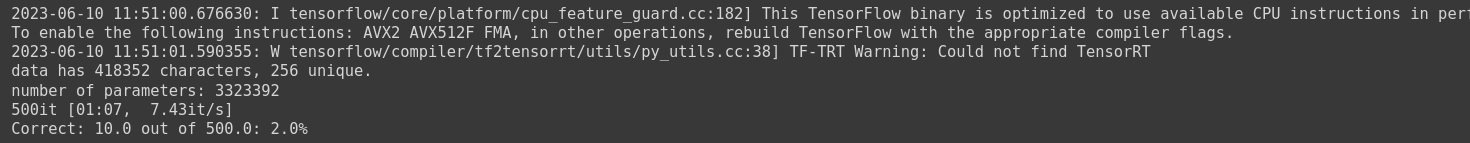
\includegraphics[width=1\textwidth]{./image/2.d.png}
    \caption{Result}
\end{figure}

London : 

\begin{figure}[ht]
    \centering
    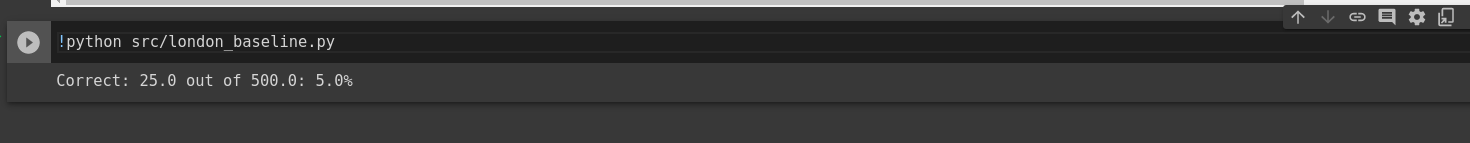
\includegraphics[width=1\textwidth]{./image/2.d.london.png}
    \caption{London result}
\end{figure}

\subsection*{e}

\begin{figure}[ht]
    \centering
    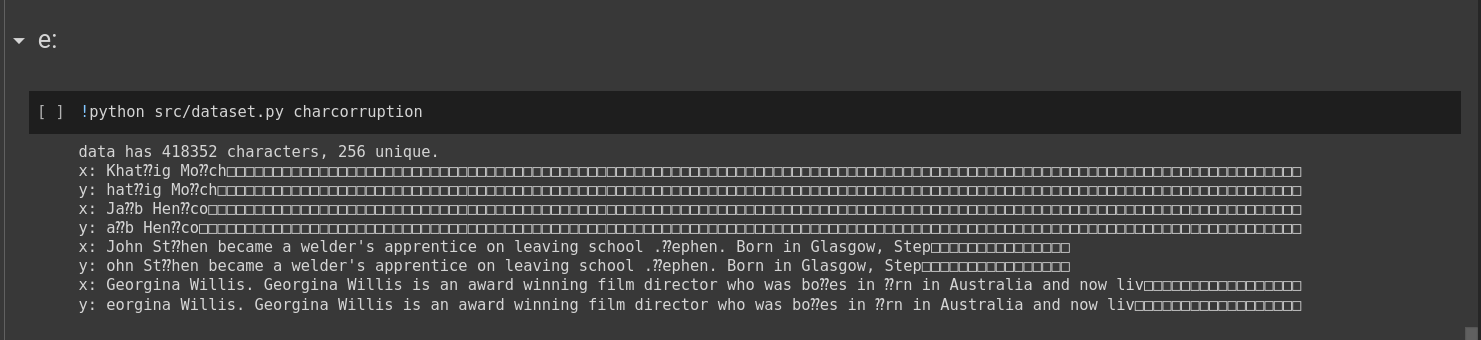
\includegraphics[width=1\textwidth]{./image/2.e.png}
    \caption{Part e result}
\end{figure}

\newpage

\subsection*{f}

\begin{figure}[ht]
    \centering
    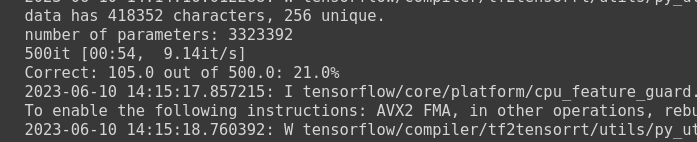
\includegraphics[width=1\textwidth]{./image/2.f.png}
    \caption{Part f result}
\end{figure}

\subsection*{g}

\begin{figure}[ht]
    \centering
    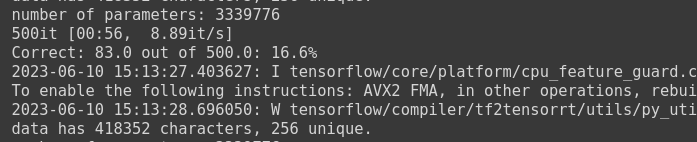
\includegraphics[width=1\textwidth]{./image/2.g.png}
    \caption{Part g result}
\end{figure}

\newpage

\section{Considerations in pretrained knowledge}

\subsection*{a.}
The pretrained model achieved an accuracy above 10\% because it had already learned the relationships between words. It gained an understanding of how different parts of a sentence depend on each other through its initial training. On the other hand, the non-pretrained model lacked this prior knowledge and was not able to grasp the intricate connections between words. Additionally, the pretrained model had the advantage of being trained on a significantly larger dataset, allowing it to potentially "memorize" the relevant aspects of the questions, further enhancing its accuracy.

\subsection*{b.}
1.The model we use sometimes can't tell if the information it gives us is true or made up. This can be a problem when people want to mention where a famous person was born. If the model gives the wrong place, people might accidentally use that wrong information in their work without realizing it's not correct. This can make their articles or research less accurate and reliable.\\

2.This issue goes beyond just one person using the model. It could lead to spreading false information in society. Imagine if people rely on the model to learn things like where famous people were born. If the model gives the wrong information and people believe it, they might unintentionally share that wrong information with others. This can cause confusion and disagreements when people start believing things that aren't true. It's important to be careful and check the information we get from the model to make sure it's right.
\subsection*{c.}

In cases where the model did not encounter a person's name during both pretraining and fine-tuning, it is impossible for the model to have "learned" where that person lived. However, the model may still generate a predicted birthplace for that person if prompted. One strategy the model might employ is to make an educated guess based on patterns and associations it has learned from similar names or contextual cues in the input text. For example, if the model has seen other famous people with similar names being associated with specific birthplaces, it might assume a similar connection for the new person's name.

This should raise concerns for the use of such applications because the model's predicted birthplace in this scenario is purely speculative and lacks any factual basis. It may provide users with potentially misleading or inaccurate information, leading to the dissemination of false facts. Relying on such speculative predictions without proper verification can result in the spread of misinformation and the erosion of trust in the application.

\end{document}